


\section*{Principio de funcionamiento}
\label{Principio de funcionamiento}

VOR es un acrónimo para la frase "\textbf{\textit{VHF Omnidirectional Range}}", que en castellano significa Radiofaro Omnidireccional de VHF. Es un tipo de radioayuda a la navegación que utilizan las aeronaves para seguir en vuelo una ruta prestablecida. Generalmente se encuentra una estación VOR en cada aeropuerto. La antena VOR de la estación emite una señal de radiofrecuencia VHF en todas direcciones, que es recibida por el equipo VOR de cualquier aeronave que se encuentre dentro del rango de alcance (max. unos 240 km) y tenga sintonizada la frecuencia de dicha estación (que puede variar de 108 a 118 MHz).

La estación de tierra posee un diagrama de radiación dinámico, transmite dos señales VHF en el rango anteriormente mencionado. La radiofrecuencia emitida por un VOR lleva tres señales codificadas. Una es la identificación de la estación en código Morse \footnote{El código Morse es un sistema de representación de letras y números mediante señales emitidas de forma intermitente.}, que permite al piloto saber de cuál estación se trata. Las otras dos son ondas senoidales de 30 Hz cuyas fases varían entre si. Se les llama señal de referencia y señal variable respectivamente. La referencia mantiene siempre su fase constante, mientras que la variable cambia su fase según la dirección en la que sea emitida. Dicha dirección se mide como un azimut, es decir, se divide en 360 grados alrededor de la antena VOR contando en sentido horario a partir del norte magnético terrestre, punto en el cual la señal de referencia y la variable tienen fase idéntica. De esta manera se puede visualizar una antena VOR como el punto desde el cual parten 360 líneas de dirección, a las que se les llama radiales.

\begin{wrapfigure}{r}{100mm}
 \centering
 \begin{center}
 \includegraphics[width=95mm]{../Imagenes/Vor_beijin.eps}
\end{center}
 \caption{D-VOR/DME ground station. Identificación "PEK" (Beijing)  \cite{VOR-Wikipedia}}
 \label{fig:Vor_de_Beijin}
\end{wrapfigure}

El equipo VOR en la aeronave recibe la señal VOR y decodifica sus tres señales. Compara la señal de referencia con la variable y determina la diferencia de fase entre las dos. De esta manera puede conocerse en qué radial del VOR sintonizado se encuentra la aeronave con respecto al norte magnético terrestre.

El VOR se utiliza en la aeronáutica para navegar según el vuelo IFR \footnote{Recibe el nombre de Reglas de Vuelo Instrumental (más conocido por sus siglas en inglés, IFR), el conjunto de normas y procedimientos recogidos en el Reglamento de Circulación Aérea, que regulan el pilotaje de aeronaves en condiciones de visibilidad reducida. Se trata del método de navegación alternativo a las Reglas de Vuelo Visual o VFR.}, siempre permaneciendo en radio con un CTA. Los VOR suelen ir acompañados de DME (Distance Measurement Equipment, Equipo de Medición de Distancia), éstos son completamente independientes del sistema VOR y ayudan al piloto a saber la distancia que hay entre la aeronave y la estación VOR. El VOR únicamente se utiliza en la llamada "radio navegación" por lo que siempre hay unos procedimientos que seguir que los marca la carta aeronáutica para dirijirse a un VOR. Por ejemplo en las SID o salidas normalizadas de un aeropuerto, en la respectiva carta se verifica el procedimiento de apoyo en la salida con los NDB y VOR para poderla realizar correctamente. El piloto debe saber volar bajo reglas de vuelo IFR a un VOR y desde un VOR, o cualquier radioayuda que sea: (NDB, VOR, ILS u otras como el TACAN \footnote{Las siglas TACAN significan  TACtical Air Navigation,  es un tipo de ayuda a la navegación de uso militar.}) \cite{VOR-Wikipedia}.

Desarrollado de un sistema anterior, Visual-Aural Range (VAR), el VOR se diseñó para proveer 360 rumos desde y hacia la estación seleccionada por el piloto. Los antiguos transmisores de tubo de vacío con antenas rotadas mecánicamente se instalaron por todos lados en la década de 1950 y en la de 1960 comenzaron a ser reemplazados por unidades de estado sólido. En este mismo período se transformaron en el mayor sistema de navegación cuando reemplazaron a las viejas radiobalizas. Algunas de estas sobrevivieron como balizas no direccionales de baja o media frecuencia (NDB \footnote{Una Baliza No Direccional,  Non-Directional Beacon (NDB), es una estación de radio ubicada en un lugar conocido, utilizada como una ayuda para la navegación aérea o naval. Como su nombre implica, la señal no provee información direccional en contraste con nuevos tipos de ayudas como VOR. La señal de una NDB copia el contorno de la curvatura de la tierra por lo que puede ser recibida a distancias mayores en latitudes menores, lo que constituye una ventaja sobre el sistema VOR. Sin embargo, la señal NDB es afectada por condiciones atmosféricas, terreno montañosos, refracción costera y tormentas eléctricas, particularmente a grandes distancias. Aún con la aparición de los sistemas VOR y GPS (Global Positioning System), las NDBs continúan siendo las ayudas de navegación más ampliamente usadas en el mundo. Las NDBs operan en el rango de frecuencias de 190 kHz a 535kHz (aunque tienen frecuencias reservadas en el rango de 190 a 1750 kHz) y una portadora modulada entre  400 o 1020 Hz \cite{NDB}. Entre la información transmitida por una NDB se tiene:

\begin{itemize}
 \item Identificación por código Morse entre 400 a 1020 Hz.
\item Información de la Terminal Aérea (Airfield Terminal Information Service = ATIS)
\item Servicio de información climática de la Terminal Aérea (Airfield Weather Information Service = AWIS), o, en una emergencia un controlador de tráfico aéreo activando la función de Presionar-para-hablar (Press-To-Talk = PTT), puede modular la portadora con la voz. El piloto utiliza su receptor ADF para escuchar las instrucciones desde la torre.
\end{itemize}
}).

En los aviones de hoy en día esto se realiza mediante la FMC, o MCDU según el fabicante del avión, ya que intoducen directamente la SID y la FMC la realiza automaticamente sola. Así podemos llevar a cabo un vuelo, tanto de larga como de corta distancia entre dos puntos del mundo.

En las rutas aéreas comerciales más transitadas, al igual que en las carreteras terrestres, hay cruces y curvas. Bajo estos ``cruces'' y ``curvas'' se suelen instalar estas estaciones VOR. Las ``carreteras aéreas'' son los radiales de XXX grados que parten de un VOR y que normalmente llegan a otro VOR o incluso a una pista de aterrizaje.

El piloto puede ordenar al piloto automático: ``\textit{Sigue el radial de 115 grados del VOR que transmite en la frecuencia 109.75 Mhz}.'', y el avión automáticamente, cuando se cruce con el radial 115, lo seguirá hasta sobrevolar el VOR.

\begin{figure} [ht]
 \centering
 \includegraphics[width=0.9\textwidth,bb=0 0 500 301]{../Imagenes/Mapa_VOR.eps}
 % Mapa_VOR.eps: 0x0 pixel, 300dpi, 0.00x0.00 cm, bb=0 0 500 301
 \caption{Mapa con ruta y posición de estaciones VOR}
 \label{Mapa_estaciones_VOR}
\end{figure}

En el mapa de la Figura  \ref{Mapa_estaciones_VOR} se puede ver una serie de radiobalizas VOR (los círculos grandes) interconectadas entre si por rutas aéreas. Cada ruta aérea tiene marcado su nombre, altitud y rumbo (que coincide con el radial del VOR del que parte).

Las distintas estaciones de VOR se clasifican por su altitud y distancia libre de interferencias a la que pueden recibir. Existen dos criterios sobre el 
particular: el americano y el de OACI.

La clasificación americana de la F.A.A es la siguiente:

%\begin{tabular}{l}{p{6cm}p{6cm}p{6cm}p{6cm}p{6cm}}
%\hline
% T-VOR. VOR : terminal &  &  &  &  \\
% L-VOR.VOR: baja altitud &  &  &  &  \\
% M-VOR.VOR: medio alcance &  &  &  &  \\
% H-VOR.VOR: gran altitud &  &  &  &  \\
%\hline 
%\end{tabular} 

Los alcances de los distintos tipos de VOR  no deben confundirse con una mayor o menor potencia de emisión de las estaciones de tierra, pues ésta es prácticamente la misma para todos, situándose alrededor  de los 200 W.

\subsection*{Precisión}
\label{sec: Presicion}
La precisión predecible de un VOR es $\pm 1,4 \deg$. Sin embargo, datos de prueba indican que el 99,94\% del tiempo con un sistema VOR tiene menos que $\pm 0,35 \deg$ de error. Los sistemas VOR son internamente monitoreados que comunican cualquier error de la estación que exceda $1,0 \deg$.

La norma ARINC 711-10 del 30 de enero de 2002 establece que la precisión del receptor debería estar dentro de $0,4 \deg$ con una probabilidad estadística del 95\% bajo varias condiciones. Cualquier receptor cumple con este estándar bien o suele excederla.

\subsection*{Futuro}
\label{sec:Futuro}

Como muchos otras formas de la navegación aérea por radio corrientemente usada, es posible que alguna forma de sistema navegacional basado en el Global Positioning System (GPS) reemplace a los sistemas VOR. VOR es específicamente lo mismo debido a que necesita numerosas estaciones cubriendo una gran área. El GPS es capaz de localizar certeramente las posiciones de aeronaves dentro de 20 m horizontalmente. El aumento de la precisión con el "Wide Area Augmentation System" (WAAS), el error se reduce a un cubo de 4 m de lado. Esta precisión instrumental se aproxima (con guías laterales y verticales) a la Categoría I de los Sistemas de Tierra. Más refinamientos incluyen el "Local Area Augmentation System" (LAAS) que probablemente certifique la Categoría III. LAAS planea usar la misma banda de frecuencia VHF para sus mensajes de corrección. Esto requerirá más facilidades de las frecuencias VOR para evitar interferencias. 



\subsection*{Sistema de tierra}
\label{Sistema_de_tierra}

\begin{figure}[h]
 	\begin{center}
 		
\includegraphics[width=0.8\textwidth]{Emisor_VOR.eps}
 % Emisor_VOR.eps: 1179666x1179666 pixel, 300dpi, 9987.84x9987.84 cm, bb=0 0 154 65
	\end{center}
 \caption{Emisor VOR situado en La Coruña, España, Tipo VOR-DME Frecuencia 115.1 MHz 
\cite{EmisorVorLaCoruniaEspania}}
 \label{Emisor_Vor}
\end{figure} 

La antena de la Figura \ref{Emisor_Vor} es una radiobaliza de tipo VOR, VHF Omnidirectional Range. Esta como otras miles similares instaladas en lugares estratégicos en todo el mundo transmite tres señales en paralelo:
\begin{itemize}
 \item Una portadora AM omnidireccional (en este caso de 115.10 MHz.) en la que se modula en morse el código de la radiobaliza (en este caso L-R-A). Puede ser captado fácilmente con cualquier radioescanner. La frecuencia de modulación es de 1020 Hz, algunos equipos tienen canales de audio que transmiten información ATIS o alguna otra para identificación.
\item En una subportadora se modula una señal de referencia de 30Hz,  también omnidireccional. 
\item En un array circular de unas 45 antenas direccionales se transmiten de forma rotatoria señales de 30 Hz (señal variable) desfasadas respeto a la señal omnidireccional de referencia. En la antena direccional que apunta hacia el Norte no está desfasada frente a la señal de referencia, la que apunta al Noreste está 45 grados desfasada, la que apunta al Este 90, Sur está 180 grados, etc...
\end{itemize}

\begin{figure}[h]
     \centering
     \subfigure[Frecuencia emisión VOR]{
          \label{fig:dl2858}
          
\includegraphics[width=.4\textwidth]{Emisor_VOR_2.eps}}
     \hspace{.3in}
     \subfigure[Array de antenas]{
          \label{fig:er2858}
          
\includegraphics[width=.4\textwidth]{Emisor_VOR_3.eps}}\\
     \vspace{.3in}
\caption{Detalles emisor VOR}
\end{figure}

 
Antiguamente, en los años 50, se utilizaban antenas que rotaban mecánicamente con un motor sus elementos direccionales.

There are two main types of VORs in operation (ie two types of actual ground installation) but the aircraft receiver is the same for both. The receiver is unaware which type of ground station is in use - it experiences the same effects from both. It's the method of creation that differs.

Existen dos tipos principales de VOR en operación, los cuales pueden observarse en la instalación de tierra pero el receptor en el avión opera de identica forma con ambos. El receptor no tiene conocimiento de cual tipo de instalación de tierra se encuentra en uso Su diferencia se encuentra en el método de creación de la señal. \ref{PrincipioOperacionEquipoTierra}

\subsubsection*{Conventional VOR - CVOR}
\label{Convencional VOR - CVOR}

The CVOR employs a rotating directional antenna. Consider for a moment a directional antenna which has a transmission pattern of one broad peak and one broad null in the horizontal plane. If we were to feed this antenna with a VHF carrier and also rotate the antenna at 30 revs/second (1800RPM) - think of how an AM receiver would view this rotation. An AM receiver would see a carrier amplitude modulated by a sine wave of 30Hz - the phase of which would be determined by the receiver's position around the station.

El CVOR emplea una antena direccional rotativa. Imagine una antena direccional que tiene un patrón de transmisión con un pico máximo y un mínimo en un plano horizontal. Si se alimenta esta antena con una señal portadora VHF y, además, se la rota a 30 revs/segundo (1800 RPM), ¿cómo percibe un receptor esta rotación de la señal? El receptor la percibe con una portadora modulada en amplitud por una onda senoidal de 30 Hz, el ángulo de fase de la cual determina la posición del receptor alrededor de la estación.

A practical CVOR doesn't actually spin the aerial at 1800RPM (although the earliest ones did!) - it uses electronic switching of an aerial array to achieve the effect. Additionally, the reference signal is transmitted by FM modulating it onto a 9960Hz subcarrier (deviation +/-480Hz). The reference signal provides the receiver its comparison to station North. The receiver compares the AM 30Hz variable phase signal recovered with the decoded 30Hz reference signal from the FM subcarrier and determines the radial position from North on which the receiver lies.

Un CVOR actual no rota la antena a 1800 RPM, en vez utiliza un arreglo de antenas para producir este efecto. Adicionalmente la señal de referencia es emitida en FM modulandola en una subportadora de 9960 Hz. La señal de referencia permite al receptor su comparación con el norte señalado por la estación

Doppler VOR - DVOR

The DVOR is a later and improved design of VOR which suffers less from siting errors. The CVOR requires a clear area of at least 1500ft in radius. The DVOR is more practical in crowded areas or where there are tall buildings. However, it's a big structure - around 100ft in diameter!

The DVOR reverses the useage of the two 30Hz signals. However, by also reversing the direction of it's rotating variable signal it produces exactly the same result in the receiver. The receiver has no "knowledge" that it's a DVOR as opposed to CVOR it's receiving and operates as normal.

In the DVOR the main VHF carrier is AM modulated at 30Hz - providing the Reference signal. This is transmitted from a central omnidirectional antenna and has the same phase all around the VOR for any receiver.

The effect of a 9960 FM modulated subcarrier is created using the Doppler effect by emplying a switched array of antenna arranged in a circle of diameter 44ft. (This distance being the exact amount to provide +/-480 apparent frequency shift in the subcarrier.)

Imagine a carrier of FcMHz AM modulated at 30Hz on the central antenna. Then imagine an array of an even number of aerial elements arranged around the cental aerial in a circle of diameter 44ft. (Typically 48 are used.) The VOR controller presents the subcarrier as sidebands on the opposite ends of an imaginary arm. Pairs of opposite aerials are switched in to form a rotating arm at 30Hz (1800RPM). The opposite aerials elements carry sidebands of (Fc+9960Hz) and (Fc-9960Hz).

From the receiver's perspective, there's a constant phase 30Hz AM modulation on the main FcMHz carrier but there also appears to be a 9960Hz subcarrier which is in turn frequency modulated at 30Hz. The sidebands will appear to be frequency modulated at 30Hz by +/-480 Hz due to the rotation and subsequent 44ft variation in distance between transmitting aerial and receiver causing Doppler Shift as the transmitting "arm" rotates. Of course, the phase of the 30Hz frequency modulation on the subcarrier (with respect to the reference signal) will depend on the receiver's angular position around the VOR. Hence, the same receiver comparison will result in the receiver's radial position being established as in the CVOR.


\subsection*{Sistema de a bordo}
\label{Sistema de a bordo}

El sistema embarcado en la aeronave está compuesto por todos los equipos que permiten la recepción y tratamiento de la onda procedente de la estación terrestre VOR, entre estos están:
\begin{itemize}
 \item Antena receptora
\item Equipo MMR, ``Multi Mode Receiver'' o Receptor Multi Modo
\item Un sistema de visualización para el piloto
\item Selector de frecuencias
\item Selector de rumbos
\end{itemize}


\subsubsection*{Antenas}
\label{Antenas}

La antena receptora es un dipolo con forma de ``V'', que recibe las ondas electromagnéticas polarizadas horizontalmente. Usualmente se ubica en el estabilizador vertical del avión o en la parte superior del fuselaje y se la carena para mejorar la resistencia aerodinámica.

\begin{wrapfigure}{r}{60mm}
 \begin{center}
 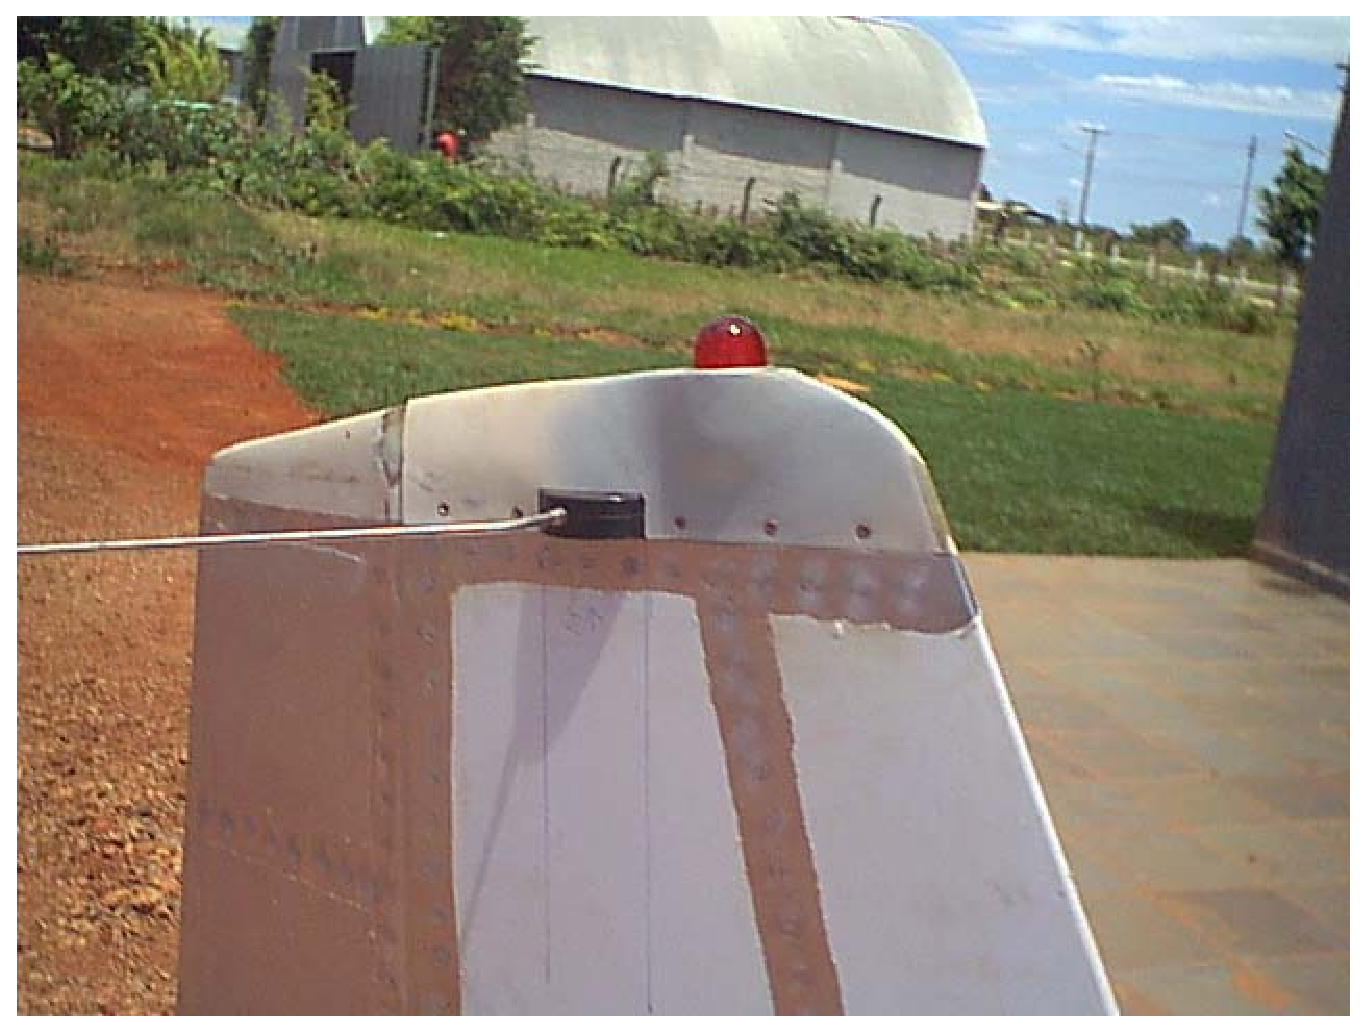
\includegraphics[width=55mm]{Antena_Vor_empenaje_vertical.eps}
 % Antena_Vor_empenaje_vertical.eps: 1179666x1179666 pixel, 300dpi, 9987.84x9987.84 cm, bb=0 0 640 480
\end{center}

\caption{Vista de una antena VOR en empenaje vertical}
\end{wrapfigure} 

Su misión consiste en captar las ondas electromagnéticas emitidas por la estación VOR, transformarlas en una señal eléctrica alterna y enviarlas por cable coaxial hasta un amplificador de señal o directamente a un receptor.

Puede darse el caso que una misma antena recepcione señales de más de un sistema de navegación. Para estos casos se coloca un duplexor para discriminarlas entre sí y enviarlas a sus receptores correspondientes.





\section*{Control del tráfico aéreo}
\label{Control_del_trafico_aereo}

El servicio de control del tráfico aéreo, también conocido por sus siglas en inglés ATC (Air Traffic Control) se presta por los países firmantes del tratado de Chicago que dieron origen a la creación de la OACI/ICAO en los términos especificados por las normas de esta organización internacional.

\begin{wrapfigure}{r}{60mm}
 \begin{center}
 \includegraphics[width=50mm]{Towers_Schiphol_small.eps}
 % Towers_Schiphol_small.eps: 0x0 pixel, 0dpi, nanxnan cm, bb=
\end{center}
	\label{Towers_Schiphol_small}
	\caption{Torre control aeropuerto Schiphol}
\end{wrapfigure}

El espacio aéreo se divide en regiones de información de vuelo, conocidas como FIR (Flight Information Region) y cada país se hace responsable del servicio en las comprendidas en su 'área de responsabilidad'. En muchos casos esta área de responsabilidad excede las aguas territoriales de un país a fin de que el espacio aéreo comprendido sobre las aguas internacionales sea provisto de un servicio de información. El espacio aéreo en el que se presta el servicio de control aéreo se llama 'espacio aéreo controlado'. La Unidad encargada de entregar el servicio de control al tráfico aéreo en estas áreas recibe el nombre de Centro de Control de Area. Debido al amplio espacio aéreo que manejan,están divididos en Sectores de Control, cada uno responsable de una parte del espacio total a su cargo. Cuando un avión está a punto de salir de un sector es traspasado al siguiente sector en forma sucesiva, hasta el aterrizaje en su destino. Actualmente, la mayor parte de las rutas aéreas están cubiertas por radares, lo que permite hacer un seguimiento permanente a los vuelos.

En las regiones de información de vuelo se encuentran las áreas terminales de los aeropuertos importantes y entre ellas discurren las aerovías, pasillos por los que circulan las aeronaves. Otros elementos son las áreas prohibidas, restringidas o peligrosas que son zonas donde el vuelo de aeronaves se ve restringido en diferentes medidas y por causas diversas.

Las normas que regulan la circulación aérea en el espacio aéreo controlado se recogen en el Reglamento de Circulación Aérea.

\newpage

\section*{DME}
\label{DME}

Distance Measuring Equipment (DME) is a transponder-based radio navigation technology that measures distance by timing the propagation delay of VHF or UHF radio signals.

It was invented by Edward George "Taffy" \ Bowen whilst employed as Chief of the Division of Radiophysics of the Commonwealth Scientific and Industrial Research Organisation CSIRO in Australia. Another Australian world-first, engineered version of the system was deployed by Amalgamated Wireless Australasia Limited in the early 1950s operating in the 200 MHz VHF band. This Australian domestic version was referred by the Federal Department of Civil Aviation as DME(D) (or DME Domestic), and the later international version adopted by ICAO as DME(I).

DME is similar to Secondary Radar, except in reverse. The system was a post-war development of the IFF (Identification Friend or Foe) systems of World War II. To maintain compatibility, DME is functionally identical to the distance measuring component of TACAN.

\subsection*{Operation}
\label{Operation}


Aircraft use DME to determine their distance from a land-based transponder by sending and receiving pulse pairs - two pulses of fixed duration and separation. The ground stations are typically colocated with VORs. A typical DME ground transponder system for enroute or terminal navigation will have a 1 kW peak pulse output on the assigned UHF channel.

A low power DME can also be colocated with an ILS localizer where it provides an accurate distance function, similar to that otherwise provided by ILS Marker Beacons.

\subsection*{Hardware}
\label{Hardware}


The DME system is composed of a UHF transmitter/receiver (interrogator) in the aircraft and a UHF receiver/transmitter (transponder) on the ground.

\subsection*{Timing}
\label{Timing}


The aircraft interrogates the ground transponder with a series of pulse-pairs (interrogations), The ground station replies with an identical sequence of reply pulse-pairs with a precise time delay (typically 50 microseconds). The DME receiver in the aircraft searches for pulse-pairs (X-mode= 12 microsecond spacing) with the correct time interval between them. The correct time between pulse pairs is determined by each individual aircraft's particular interrogation pattern. The aircraft interrogator locks on to the DME ground station once it understands that the particular pulse sequence is the interrogation sequence it sent out originally. Once the receiver is locked on, it has a narrower window in which to look for the echoes and can retain lock.

\subsection*{Distance calculation}
\label{Distance calculation}


A radio pulse takes around 12.36 microseconds to travel one nautical mile to and from, this is also referred to as a radar-mile. The time difference between interrogation and reply minus the 50 microsecond ground transponder delay is measured by the interrogator's timing circuitry and translated into a distance measurement in nautical miles which is then displayed in the cockpit.

\subsection*{Specification}
\label{Specification}


A typical DME transponder can provide concurrent distance information to about 100 aircraft.[1] Above this limit the transponder avoids overload by limiting the gain of the receiver. Replies to weaker more distant interrogations are ignored to lower the transponder load.

\subsection*{Radio frequency and modulation data}
\label{Radio frequency and modulation data}


DME frequencies are paired to VHF omnidirectional range (VOR) frequencies. A DME interrogator is designed to automatically tune to the corresponding frequency when the associated VOR is selected. An airplane’s DME interrogator uses frequencies from 1025 to 1150 MHz. DME transponders transmit on a channel in the 962 to 1150 MHz range and receive on a corresponding channel between 962 to 1213 MHz. The band is divided into 126 channels for interrogation and 126 channels for transponder replies. The interrogation and reply frequencies always differ by 63 MHz. The spacing of all channels is 1 MHz with a signal spectrum width of 100 kHz.

Technical references to X and Y channels relate only to the spacing of the individual pulses in the DME pulse pair, 12 microsecond spacing for X channels and 36 microsecond spacing for Y channels.

DME facilities identify themselves with a 1350 Hz morse code three letter identity. If collocated with a VOR or ILS it will have the same identity code as the parent facility. Additionally, the DME will identify itself between those of the parent facility. DME identity is 1350 Hz to differentiate itself from the 1020 Hz tone of the VOR or the ILS localizer.

\subsection*{Accuracy}
\label{Accuracy}


Accuracy of DME is 185 m ($\pm 0.1 \ nm $).[1] One important thing to understand is that DME provides the physical distance from the aircraft to the DME transponder. This distance is often referred to as 'slant range' and depends trigonometrically upon both the altitude above the transponder and the ground distance from it.

For example, an aircraft directly above the DME station at 6000 feet altitude would still show one mile on the DME readout. The aircraft technically is a mile away, just a mile straight up. Slant range error is most pronounced at high altitudes when close to the DME station.

\subsection*{Future}
\label{Future}


It is likely that DME installations will be phased out when space based navigational systems such as GPS and Galileo become widely used for aviation.[2] However, the system is still widely used and new beacons are being built and installed still today (June 2007).


Las siglas TACAN significan  tactical air navigation, y este es un tipo de ayuda

a la navegación de uso militar.

La información que proporciona al piloto es la de azimut y la distancia  con

respecto a la instalación de tierra, dando pues, en cada instante, la posición

del avión.

El equipo de tierra esta constituido por un receptor- transmisor y una antena

giratoria para la transmisión de información de marcaciones magnéticas y la

distancia. La distancia la recibe el piloto a trabes de su equipo radio

telemétrico (DME).

El TACAN trabaja en UHF y puede ser sintonizado en uno de los 126 canales que le

han sido asignados a este tipo de radioayuda. Los canales van espaciados 0.5

Mhz.

La identificación de las estaciones TACAN es auditiva, en código MORSE, y esta

compuesta por tres letras que se repiten una vez cada 30 segundos.

La cobertura del equipo es similar a la del VOR y su exactitud puede calibrarse

en $\pm- 1 $.

El cono de silencio en los TACAN es muy grande, del orden de 13 o 15 NM a

40.000. por ello, y para evitar errores, únicamente se considera pasada la

estación, cuando el equipo DME indique un incremento de distancia.

Los indicadores de abordo que usa el equipo TACAN, son los mismos que los

utilizados para el VOR.

SISTEMA VORTAC

El VORTAC es una radioayuda que combina las funciones del VOR y de los TACAN, y

transmite información en azimut en VHF y UHF y de distancia en UHF. De esta

manera tanto las aeronaves equipadas con VOR, DME, TACAN, recibirán información

de azimut y distancia al VORTAC.

SISTEMA LORAN

El long range navigation, LORAN es un sistema de navegación hiperbólica

radioeléctrico e largo alcance, que opera en baja y media frecuencia.

Este equipo proporciona información de posición midiendo la diferencia de tiempo

en microsegundos, entre la llegada de dos señales de radio desde dos estaciones

transmisoras de tierra.

Para navegar con el sistema LORAN es necesario sintonizar dos grupos de

estaciones en tierra. Cada uno de ellos esta constituido por dos equipos

emisores que reciben el nombre de estación primaria y estación secundaria.

Lógicamente, cada grupo de estaciones LORAN emitirá en frecuencias distintas.

Centrándose el estudio en uno de los grupos transmisores, el proceso seguido es

el siguiente: la estación principal del grupo LORAN emite ondas

electromagnéticas de radio que son captadas por el avión y por la estación

secundaria, la cual envía sus propias señales hacia la aeronave.

Las señales que lanza la estación  principal llegan al equipo de abordo antes

que las de la estación secundaria, con una diferencia de tiempo tal, que

dependerá de la posición del avión. El receptor LORAN analizara la diferencia de

tiempo entre las dos señales.

Esa diferencia de tiempo determinara una línea sé situación que debido a la

posición  relativa de las estaciones principal y secundaria, y al recorrido que

deba efectuar las ondas hasta llega al avión, tendrá la forma e una hipérbola.

La aeronave puede estar situada en cualquier punto de la hipérbola. Pues en cada

uno de sus puntos, la diferencia de tiempo en la llegada de las señales de las

estaciones  LORAN, es constante.

Para conocer exactamente la posición del avión sobre la hipérbola será necesario

sintonizar otro grupo LORAN para llevar a cabo el mismo procedimiento. Una vez

hallada la nueva diferencia de tiempos, sobre la carta de navegación, podrá

buscarse otra línea hiperbólica, correspondiente al grupo últimamente

sintonizado, que este de acuerdo con la diferencia de tiempos determinada por el

receptor de a bordo.

El equipo LORAN consiste en una receptor de baja y media frecuencia y una

pantalla de rayos catódicos en la cual aparecen  una serie de líneas producidas

por la recepción en el avión de las ondas lanzadas desde tierra. Con una

plantilla especial se mide la diferencia de tiempos ente las señales

representadas en la pantalla.
